% The listwise prompt, simplified. Shared by the technical report (Figure 2) and the repository README
% (rendered to PNG). The exact prompt: prompt A in the report's appendix, built by listwise_rerank/ranker.py.
% Example: the ViDoRe V3 instruction and an illustrative query. The thumbnails and bar heights are not data.
\documentclass[tikz, border=0pt]{standalone}
\usepackage[T1]{fontenc}
\usepackage[type1, sfdefault]{noto-sans}
\usepackage[type1, scale=0.92]{noto-mono}
\usetikzlibrary{arrows.meta, positioning, calc, shadows.blur}
% Colours, the gradient and the target icon shared by the report style and the standalone figures.
% \input by techreport.sty users and by the standalone figures. Needs xcolor and tikz.
\definecolor{jevink}{HTML}{1F1F1F}
\definecolor{jevmuted}{HTML}{444746}
\definecolor{jevsubtle}{HTML}{5E6368}
\definecolor{jevline}{HTML}{DDE3EA}
\definecolor{jevline2}{HTML}{E3E8EF}
\definecolor{jevfill}{HTML}{F0F4F9}
\definecolor{jevground}{HTML}{F8FAFD}
\definecolor{jevlink}{HTML}{0B57D0}
\definecolor{jevblue}{HTML}{4285F4}
\definecolor{jevpurple}{HTML}{9B72CB}
\definecolor{jevrose}{HTML}{D96570}
\definecolor{jevred}{HTML}{EA4335}
\definecolor{jevyellow}{HTML}{FBBC04}
\definecolor{jevgreen}{HTML}{34A853}
\pgfdeclarehorizontalshading{jevgrad}{100bp}{color(0bp)=(jevblue); color(25bp)=(jevblue); color(52bp)=(jevpurple);
  color(75bp)=(jevrose); color(100bp)=(jevrose)}
% the target icon, at height #1
\newcommand{\jevtarget}[1]{%
  \tikz[baseline=-0.5ex]{\draw[jevrose, line width=#1*0.12] (0,0) circle[radius=#1*0.38]; \fill[jevrose] (0,0) circle[radius=#1*0.18];}}

\newcommand{\semib}{\fontseries{sb}\selectfont}
% a page thumbnail centred at (#1,#2): accent colour #3, layout #4 (0 text, 1 chart, 2 table, 3 figure)
\newcommand{\pagethumb}[4]{%
  \begin{scope}[shift={(#1-0.31,#2-0.41)}]
    \draw[jevline, fill=white, line width=0.5pt, rounded corners=1.5pt] (0,0) rectangle (0.62,0.82);
    \fill[#3, rounded corners=0.6pt] (0.09,0.68) rectangle (0.38,0.73);
    \ifcase#4
      \foreach \yy in {0.56,0.47,0.38,0.29,0.20} \fill[jevline, rounded corners=0.5pt] (0.09,\yy) rectangle (0.53,\yy+0.045);
    \or
      \fill[jevline, rounded corners=0.5pt] (0.09,0.56) rectangle (0.53,0.605);
      \foreach \xx/\hh in {0.11/0.14,0.21/0.25,0.31/0.19,0.41/0.31} \fill[#3!50] (\xx,0.12) rectangle (\xx+0.07,0.12+\hh);
    \or
      \fill[jevline, rounded corners=0.5pt] (0.09,0.56) rectangle (0.40,0.605);
      \draw[jevline, line width=0.4pt] (0.09,0.12) rectangle (0.53,0.47) (0.09,0.355) -- (0.53,0.355)
        (0.09,0.24) -- (0.53,0.24) (0.25,0.12) -- (0.25,0.47);
    \or
      \fill[jevfill] (0.09,0.32) rectangle (0.53,0.61);
      \foreach \yy in {0.22,0.13} \fill[jevline, rounded corners=0.5pt] (0.09,\yy) rectangle (0.53,\yy+0.045);
    \fi
  \end{scope}}
\begin{document}
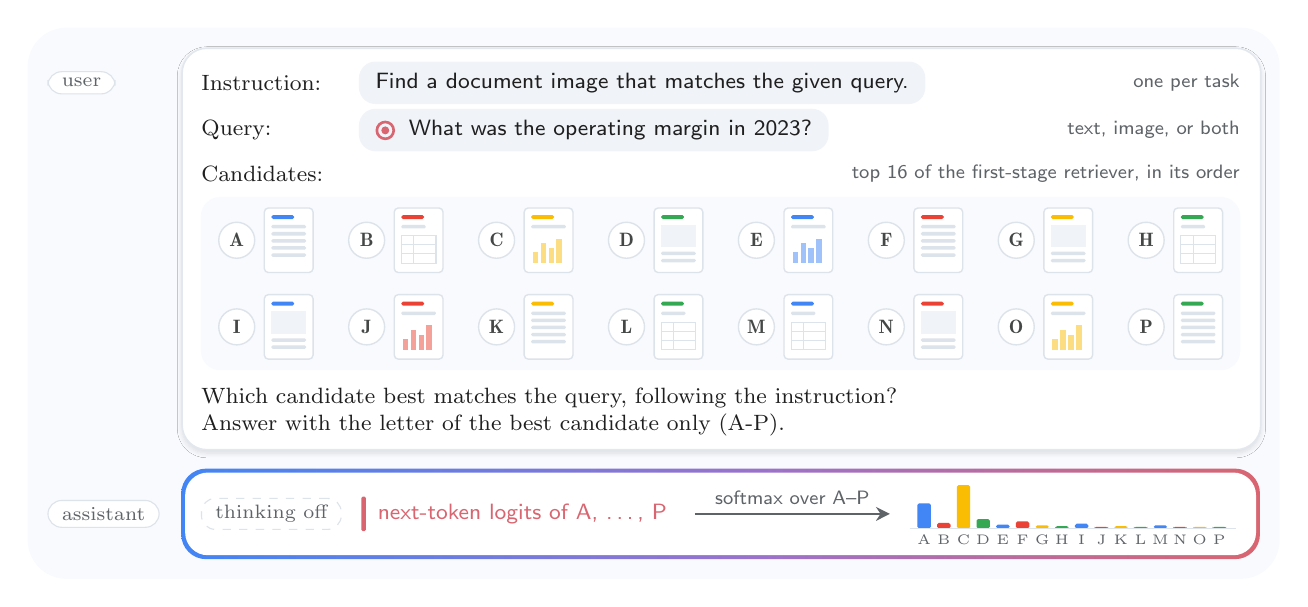
\begin{tikzpicture}[
    font=\sffamily\small, text=jevink,
    card/.style={fill=white, draw=jevline2, line width=0.6pt, rounded corners=9pt,
                 blur shadow={shadow blur steps=8, shadow xshift=0pt, shadow yshift=-1.2pt, shadow opacity=12}},
    chip/.style={fill=jevfill, rounded corners=6pt, inner xsep=6pt, inner ysep=0pt, minimum height=0.54cm,
                 font=\sffamily\fontsize{7.6}{9}\selectfont, anchor=west},
    lit/.style={font=\notomono\footnotesize, text=jevink, inner sep=0pt, anchor=west},
    role/.style={draw=jevline, fill=white, rounded corners=5pt, inner xsep=5pt, inner ysep=2.5pt, anchor=west,
                 font=\notomono\scriptsize, text=jevsubtle},
    lab/.style={circle, minimum size=13pt, inner sep=0pt, font=\notomono\scriptsize\semib, fill=jevfill, text=jevmuted},
    note/.style={font=\sffamily\scriptsize, text=jevsubtle, inner sep=0pt},
    flow/.style={-{Stealth[length=5pt, width=5pt]}, line width=0.9pt, draw=jevsubtle},
  ]
  % ---------------------------------------------------------------- canvas
  \fill[jevground, rounded corners=14pt] (0,0) rectangle (15.9,7.0);

  % ---------------------------------------------------------------- user turn
  \node[role] at (0.25,6.3) {user};
  \node[card, minimum width=13.7cm, minimum height=5.1cm, anchor=north west] at (1.95,6.75) {};
  \node[lit] at (2.2,6.3) {Instruction:};
  \node[chip] (ins) at (4.2,6.3) {Find a document image that matches the given query.};
  \node[note, anchor=east] at (15.4,6.3) {one per task};
  \node[lit] at (2.2,5.7) {Query:};
  \node[chip] (q) at (4.2,5.7) {\jevtarget{8pt}\hspace{5pt}What was the operating margin in 2023?};
  \node[note, anchor=east] at (15.4,5.7) {text, image, or both};
  \node[lit] at (2.2,5.15) {Candidates:};
  \node[note, anchor=east] at (15.4,5.15) {top 16 of the first-stage retriever, in its order};
  % the 16 candidates, each introduced by its label
  \fill[jevground, rounded corners=7pt] (2.2,2.65) rectangle (15.4,4.85);
  \foreach \L/\c/\v [count=\i from 0] in {A/jevblue/0, B/jevred/2, C/jevyellow/1, D/jevgreen/3, E/jevblue/1, F/jevred/0,
      G/jevyellow/3, H/jevgreen/2, I/jevblue/3, J/jevred/1, K/jevyellow/0, L/jevgreen/2, M/jevblue/2, N/jevred/3,
      O/jevyellow/1, P/jevgreen/0} {
    \pgfmathsetmacro\x{2.2 + 0.225 + mod(\i,8)*1.65}
    \pgfmathsetmacro\y{\i < 8 ? 4.3 : 3.2}
    \node[lab, fill=white, draw=jevline, line width=0.5pt] at (\x+0.23,\y) {\L};
    \pagethumb{\x+0.89}{\y}{\c}{\v}
  }
  \node[lit] at (2.2,2.3) {Which candidate best matches the query, following the instruction?};
  \node[lit] at (2.2,1.95) {Answer with the letter of the best candidate only (A-P).};

  % ---------------------------------------------------------------- assistant turn: read, do not decode
  \node[role] at (0.25,0.825) {assistant};
  \shade[shading=jevgrad, rounded corners=9pt] (1.95,0.25) rectangle (15.65,1.4);
  \fill[white, rounded corners=8.2pt] (2.0,0.3) rectangle (15.6,1.35);
  \node[role, draw=jevline, dashed] (th) at (2.2,0.825) {thinking off};
  \fill[jevrose, rounded corners=0.5pt] ($(th.east)+(0.25,-0.22)$) rectangle ++(0.055,0.44);
  \node[anchor=west, font=\sffamily\footnotesize, text=jevrose, inner sep=0pt] (rd) at ($(th.east)+(0.45,0)$)
       {next-token logits of A, \dots, P};
  \draw[flow] ($(rd.east)+(0.35,0)$) -- node[note, above=3pt] {softmax over A--P} (10.95,0.825);
  % one probability per candidate, coloured as its thumbnail
  \foreach \L/\c/\h [count=\i from 0] in {A/jevblue/0.32, B/jevred/0.07, C/jevyellow/0.55, D/jevgreen/0.12, E/jevblue/0.05,
      F/jevred/0.09, G/jevyellow/0.04, H/jevgreen/0.03, I/jevblue/0.06, J/jevred/0.02, K/jevyellow/0.03, L/jevgreen/0.02,
      M/jevblue/0.04, N/jevred/0.02, O/jevyellow/0.02, P/jevgreen/0.02} {
    \fill[\c, rounded corners=0.6pt] (11.3+\i*0.25,0.64) rectangle ++(0.17,\h);
    \node[font=\notomono\fontsize{5}{6}\selectfont, text=jevsubtle] at (11.385+\i*0.25,0.5) {\L};
  }
  \draw[jevline] (11.2,0.64) -- (15.35,0.64);
  % report the right edges that must stay inside the cards (inner right edge 15.4 cm)
  \path (ins.east); \pgfgetlastxy{\ex}{\ey}\typeout{EDGE ins=\ex}
  \path (rd.east); \pgfgetlastxy{\ex}{\ey}\typeout{EDGE rd=\ex}
\end{tikzpicture}
\end{document}
